\documentclass[a4paper,onecolumn]{report}
\usepackage{caption}
\usepackage{subcaption}
\usepackage{setspace}
\usepackage{amssymb}
\usepackage[fleqn]{amsmath}
\usepackage{apacite}
\usepackage{graphicx}
\usepackage{color}
\usepackage{float}
\usepackage[toc,page]{appendix}
\usepackage[nottoc]{tocbibind}
\usepackage{titlesec}
\usepackage{float}
\usepackage{color}
\usepackage{setspace}
\usepackage{comment}
\usepackage{url}
\titleformat{\chapter}{\normalfont\huge}{\thechapter.}{15pt}{\huge}
\renewcommand*{\familydefault}{\sfdefault}
\hyphenpenalty=5000 
\tolerance=1000

\usepackage[a4paper]{geometry}
\voffset=-80pt
\hoffset=0pt
\topmargin = 0pt
\textwidth = 450pt
\textheight = 770pt
\marginparwidth = 10pt
\oddsidemargin = 5pt
\topmargin = 1pt
\graphicspath{ {/images/} }

\setcounter{tocdepth}{2}

\begin{document}

%----------------------------------------------------------------------------------------
%	TITLE SECTION
%----------------------------------------------------------------------------------------

\begin{titlepage}

\newcommand{\HRule}{\rule{\linewidth}{0.5mm}}
\newcommand{\horrule}[1]{\rule{\linewidth}{#1}}

\center % Center everything on the page

\textsc{\small DELFT UNIVERSITY of TECHNOLOGY}\\[2.5cm] % Name of your university/college

\textsc{\LARGE Artificial Neural Networks}\\[0.5cm] % Major heading such as course name

\HRule \\[0.1cm]
\begin{spacing}{1.6}
{ \huge PROJECT REPORT}\\[-0.4cm] % Title of your document
\end{spacing}
\HRule \\[1.5cm]

\begin{minipage}{0.4\textwidth}
\begin{flushleft} \large
\emph{Authors:}\\
Michiel \textsc{Bongaerts\\}
Marjolein \textsc{Nanninga}\\
Tung \textsc{Phan}\\
Maniek \textsc{Santokhi}
\end{flushleft}
\end{minipage}
~
\begin{minipage}{0.4\textwidth}
\begin{flushright} \large
\end{flushright}
\end{minipage}\\[4cm]

{\large \today}\\[3cm]


\vfill

\end{titlepage}

%----------------------------------------------------------------------------------------
%	CONTENT
%----------------------------------------------------------------------------------------

\tableofcontents

\chapter{Introduction}

Mapping the world around us has always been a human endeavour to advance economical output. A better understanding of the places around us makes for more efficient traveling and exploitation of the land. However, it has always been a very slow and tedious process to produce these maps, something technology has not changed just yet.

A new opportunity has arisen with the arrival of satellite imagery and an ever increasing amount of computational power. An opportunity where this mapping can be done automatically so that this tedious and slow job can be processed even more quickly and perhaps more accurately. It is with this in mind we further analyse any possibilities.\\
\\
This paper proposes an update. Now a more straightforward approach has been chosen in which the emphasis lies on the actual Neural Network rather than the conversion of interpreted images to vector graphic maps. The new approach deals with image patches rather than pixels. This document discusses the newly acquired concept with a list of features and the actual implementation details. Also an updated schedule will be presented. 

\chapter{Concept}
Earlier attempts to conceptualise the idea to automate map making resulted in a proposal that too heavily focused on the actual map creation rather than the classification. For a Neural Network course this was deemed not befitting enough. The plan was also quite far reaching to start with. Thoughts were put into downscaling this ambitious plan. We played around a bit and came up with a new concept which will be discussed in this chapter. Firstly, an impression is given how the end user interacts with our system. This will lay the groundwork for how the Neural Network will be constructed. Secondly through the principles of MoSCoW a flexible requirements list is established. Actual talk about the classification is done in the subsequent chapter.

\section{Impression}

Below in figure \ref{fig:impression} an impression is given of what the end user will interact with and a possible result that might come about from said interaction.\\

\begin{figure}[h!]
    \centering
    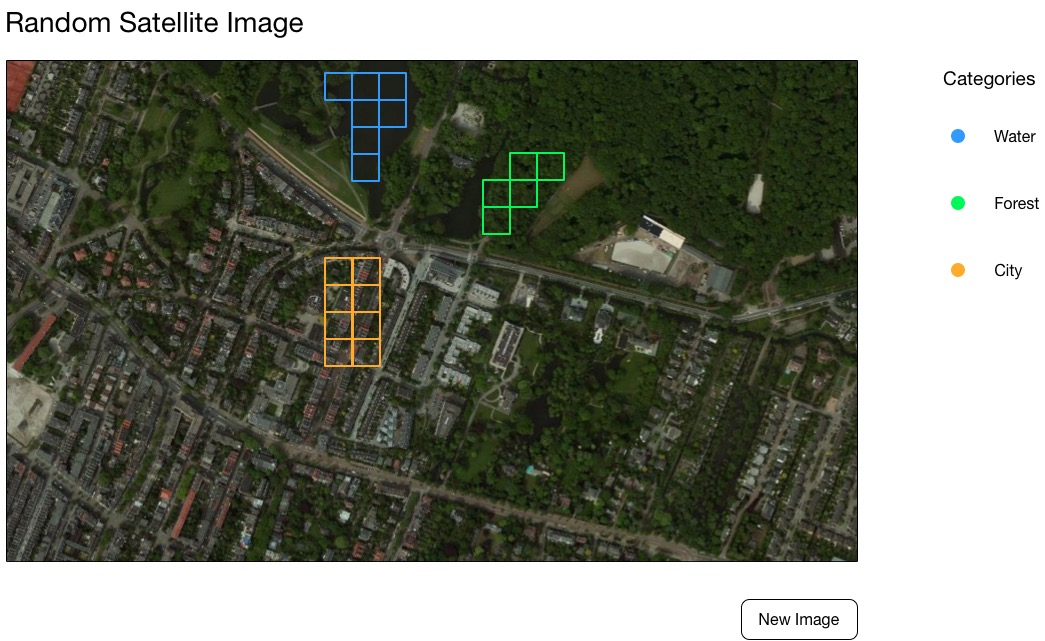
\includegraphics[width=0.8\textwidth]{./images/impression.jpg}
    \caption{Impression of what the user interacts with and a possible outcome.}
	\label{fig:impression}
\end{figure}
\noindent
The most notable attention grabber is the satellite image. This image will be acquired through a random call from a homogeneous satellite image database on every new instantiation of the system. Another possibility to acquire new data is by clicking on the 'New image' button. Right of the satellite image one can see labels (Forest, City, Water) which correspond with the labels which are outputs of the classification. Results obtained from our algorithm, given the current satellite image as input, are graphically feed back to the user. The impression above does that by showing a correspondence between image patches and their respective label via color coding laid over the satellite image. This rendition just shows a few islands of results as an example. Normally the entire image will have such arching (which will be a lot more subtle).\\
\\
Figure \ref{fig:grid} shows how it works internally. Two grids are maintained. One with patches the size of 25 by 25 pixels. The other by the size of 50 by 50 pixels. The latter is actually fed to the Neural Network from which will be decided for that patch the percentage of type of label it contains.  Four 50 by 50 pixels will be grouped together to create a square. In the middle the 25 by 25 pixels patch is placed. This patch will eventually be coloured on the satellite image to indicate the type of label. To decide that, a weighted majority vote of the four 50 by 50 pixels surrounding that smaller patch is computed. Like a convolution filter this construction is shifted over the satellite image as to decide for every area on it. As one can imagine, 25 pixels at the borders are omitted. 

\begin{figure}[h!]
    \centering
    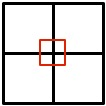
\includegraphics[scale=0.6]{./images/grid.jpg}
    \caption{Grid structure which facilitates the algorithm.}
	\label{fig:grid}
\end{figure}

\section{MoSCoW}
Since our time to work on this project is limited while the amount of goals we wanted to accomplish in this period were numerous, we used the MoSCoW analysis technique to get prioritize these goals and focus on the most important requirements. MoSCow stands for \textit{Must have}, \textit{Should have}, \textit{Could have} and \textit{Would have}, with the importance of each category ordered in a descending fashion. This enables us to identify core requirements which are absolutely necessary for the functionality of our implementation and in turn enables us to set up the core functionality first before focusing on the secondary objectives. All the requirements are labeled in these four classes.\\

\subsection{Must have}
Must have requirements are critical to project success. 
\begin{itemize}
\item Create code based on a \textit{Convolutional Neural Network} (CNN) that enables automatic classification of patches from satellite images. Considering images acquired on provincial level and a substantial amount of pixels in one patch (at least 50 x 50 pixels). 
\item At least the following classes should be recognized: vegetation, city and water. 
\item Develop a way to visualize the automatic classifications clearly.
\end{itemize}

\subsection{Should have}
Requirements labeled as should have are important to book success, but not necessary for delivery. 

\begin{itemize}
\item Create a clear interface in which the unlabeled images can be uploaded, and the output consists of labeled images. 
\item Calculate the uncertainty in the classification and ask user input for very uncertain patches.
\end{itemize}

\subsection{Could have}
It would be very nice if we would be able to reach the Could have features, but they are not critical. 
\begin{itemize}
\item Experiment with preprocessed images (noise reduction, gradient calculations)
\item Analyze images on city level, so with more details present. For this purpose new classes have to be added, such as roadways, cycle paths, 	buildings, distinct vegetations etc. 
\item Experiment with other models than the state-of-the art LeNet-1 CNN. For examples, a CNN in which Genetic Algorithms are incorporated, or implementing an Extreme Learning Machine for the training of the weights. 
\end{itemize}

\subsection{Would have}
These requirements are implemented only in the most ideal situation. They are considered as the dream project, sometimes serving as a suggestion for further projects. 

\begin{itemize}
\item Develop a method for high-detailed automatic vector graphics, in which segmentation of the distinct labeled classes is incorporated.
\item Use the input of the users to improve the automatic classification. 
\item Sell the software package to Google. 
\end{itemize}

\subsection{Elaboration on the design choices}
As the name of the Must have category implies, these requirements are critical to the success of the project and as such, these requirements were all met. The CNN is designed and is trained beforehand, the resulting weights are then injected into the CNN placed on the server, used to classify the map patches. The CNN is capable of distinguishing three separate classes, with an experimental CNN capable of distinguishing four classes (further elaborated in Section \ref{sec:resultsanddiscussion}).
A basic web interface was created, with the ability to highlight specific classes to help visualize the classification of the network.

Due to time constraints, some requirements had to be modified in order to implement them or were left out altogether. The ability to upload own satellite imagery was replaced with the ability to acquire random satellite imagery of Amsterdam and its surroundings, which are in turn classified by the network. Choosing this route means that we do can worry less about content validity and security of the application.

The calculation of uncertainty is possible, but the implementation of user correction in conjunction with this uncertainty was left out. This is due to time constraints and the fact that we have not implemented on-line learning, but rather let the network train off-line beforehand, making this feature obsolete.

Preprocessing the images could have been implemented and would surely boost our classification results. However, the goal of this project was not to achieve a high classification performance, but rather to implement a neural network that could learn on its own what the best discriminating features of an image is.

The option to classify maps on different altitude levels is not implemented, also due to time constraints. Different levels of altitude means to either have a general neural network that works on all altitudes, or having to train the network on different altitudes in order to produce multiple weight setups. Both of these options meant more time needed to develop, implement and test the new setups. 

Different setups have been experimented with, which will be discussed in Section \ref{sec:resultsanddiscussion}.

The would haves requirements were on a whole different level and thus are self-explanatory why they weren't implemented.



\chapter{Implementation}
A plan has been established what kind of application should come about. The previous discussion pressed for a certain kind of structure. One where a Neural Network is central to the problem to be solved. But also a frontend is needed for certain user interaction as well as an infrastructure in the backend which facilitates the communication with said frontend. This chapter discusses these aspects.

\section{Frontend and Backend}
The impression given above in figure \ref{fig:impression} is close to what the end result should look like (although it only displays a certain state). Yet an entire infrastructure outside of the Neural Network is needed to facilitate the application. Below in figure \ref{fig:communication} an infrastructure is visualised via the communication of the two entities.

\begin{figure}[h!]
    \centering
    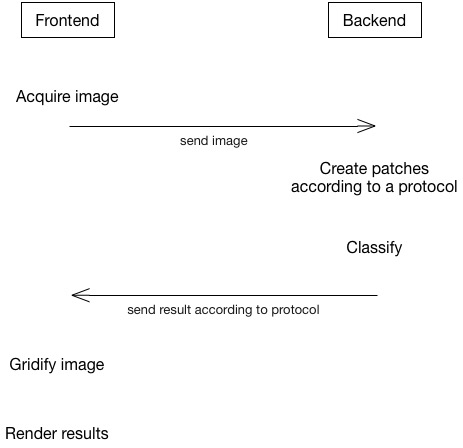
\includegraphics[scale=0.5]{./images/communication.jpg}
    \caption{Communication visualisation between frontend and backend.}
	\label{fig:communication}
\end{figure}
\noindent
First, at the frontend, an image is acquired by the user from a database call. The image is immediately send to the backend. There, patches are extracted according to a certain protocol (specific size and sequence). The patches are classified by our Neural Network. Send back to the frontend are the results in a list according to the sequence defined by the protocol. Also a codification of the results is part of the protocol. Back at the frontend the image is made into a grid which corresponds to the size of the protocol. According to the results of the Neural Network these grid windows are coloured.

\section{Dataset}
The image which is being acquired every time comes from the Bing Maps database \cite{bing}. A predefined size of the map with satellite view enabled, the labels turned off, no other controls or logos visible and where the hight is 100 meters is put in the frontend.  Randomly a location inside the Netherlands is generated. Now the actual image is taken from the map.

For training, satellite images from the same source and practice mentioned above are drawn on a per category/label basis. Patches are acquired code-wise over those images so that for each patch it is known what category/label belongs to it.


\chapter{Convolutional Neural Network}
\label{chap:CNN}
During our research phase, we encountered a variety of papers that describes the use of image classification based on Neural Networks. Most of these papers have one thing in common which is the use of Convolutional Neural Networks (CNN). Since convolution operations are widely used to extract features from images and since these operations can be represented in terms of a Neural Network these properties lead to the existence of the Convolutional Neural Networks. 
\\\\
In general a CNN architecture consist of multiple Convolution layers and sub-sampling layers. It depends on the architecture how these layers are followed by each other. The convolution layer is the layer which results after the convolution operator is performed by the a convolution kernel. Since the gaol is to extract general features from our input image we want the CNN to generalize. This generalization is partly released by dimension reduction. Since convolution operation reduce the dimension of our input map with $\frac{M-N+1}{M}$, where $N$ is the dimension of the convolution kernel and $M$ the dimension of the input map, we want the dimension to be reduced more quickly. This is done by dub-sampling kernels which in general 'squeeze' or average the input map with a certain dimension. This operation is equivalent to a convolution operation but with a larger step-size (convolution uses a step size equal to 1) and equal weights for each element in the sub-sampling kernel.

\section{LeNet-1}
The model we implement is LeCun's LeNet-1 \cite{lenet}. This model uses an alternating sequence of convolution and sub-sampling layers. The architecture of this network is shown in Figure \ref{fig:Architecture}. The convolution layers act as feature maps, they consist of a window of a certain size, whose pixels are trainable weights. The sub-sampling layers reduce the dimensionality of the outputs. 
\begin{figure}[h!]
    \centering
    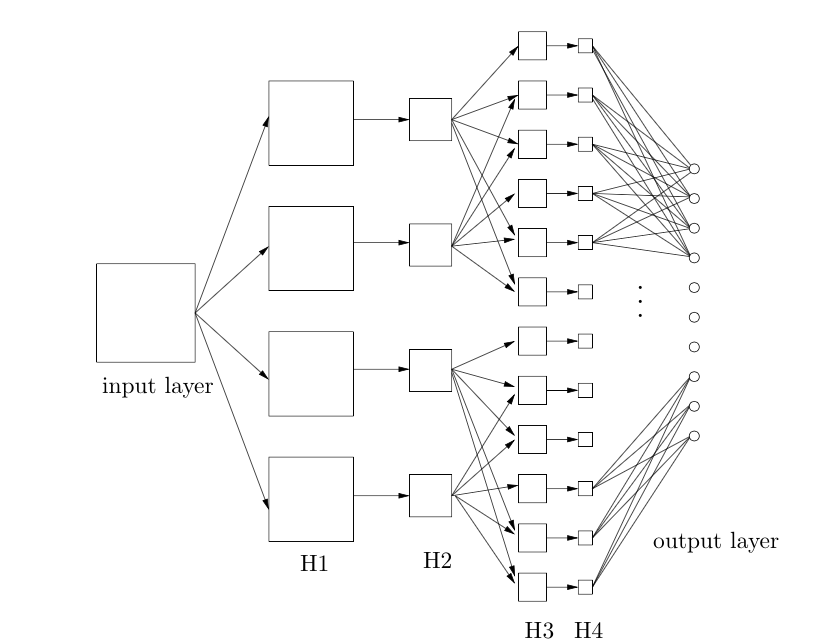
\includegraphics[scale=0.4]{./images/Architecture_CNN.png}
    \caption{The architecture of the CNN proposed by LeNet. H1 and H3 are the convolution layers, H2 and H4 the sub-sampling layers to reduce the dimension. }
	\label{fig:Architecture}
\end{figure}
\\\\
One of the biggest advantages of using CNN, and especially LeCun's LeNet-1 implementation, is the incorporation of back-propagation learning. Meaning that all the weights of the layers are adjusted iteratively, eliminating the need to manually create the convolution masks.
\\
\section{Back-propagation}
\label{sec:BP}
To train the network we have to adjust several parameters in the network. In this research we consider back-propagation from layer output to H4 to H3. In the whole network we use the Sigmoidal activation functions which is given by:
\begin{equation}
f(x)=\frac{1}{1+e^{-x}} 
\end{equation}	
The error function is defined as:
\begin{equation}
E=\sum_{k} \frac{1}{2}|t_k-F_{k}|^{2}
\end{equation}
Where $t_k$ represent the labeled class of the training. This variable is $1$ if the corresponding class is trained and $0$ if this is not the case. Below the functions are listed in which we go from the activation of our classifier neuron to value obtained in layer H3. In these equations $r$ stands for row which is the first branch after the first convolution i.e. the total rows is equal to the amount of different feature maps in H1. $b$ stands for the amount of branches per row. $k$ stands for the amount of classes which are trained by the network.
\begin{equation}
\begin{split}
	&F_{k}= f( x_{k}) \\
	& x_{k}=\sum_{ij} W^{4rbk}[i,j] \; H^{4rb}[i,j] - b_{k} \\
	&H^{4rb}[i,j]= \sum_{u,v} W^{3rb}[u,v] \; H^{3rb} [2i+u,2j+v] \\
	&H^{3rb} [2i+u,2j+v]= f\left (x^{3rb}[2i+u,2j+v] \right) \\
	&x^{3rb}[2i+u,2j+v]=\sum_{nm} W^{2rb}[n,m] \; H^{2rb}[n+(2i+u),m+(2j+v)] -b^{3rb}
\end{split}
\end{equation}
From these equations we can calculate the update-rules for back-propagation. This is done by applying the gradient descent method in which we calculate the derivatives of out error function. The update-rule consists of the derivative with respect to the parameter we want to update with some 

\begin{equation}
\begin{split}
\Delta W^{4rbk}[i,j]&= \sum_{k} - \eta \frac{dE}{d F_{k}} \frac{dF_{k}}{dx_{k}} \frac{dx_{k}}{dW^{4rbk}[i,j]} \\
&= \sum_{k} \eta (t_{k}-F_{k})\frac{e^{-x_{k}}}{(1+e^{-x_{k}})^{2}} \frac{dx_{k}}{dW^{4rbk}[i,j]} \\
&= \eta (t_{k}-F_{k})\frac{e^{-x_{k}}}{(1+e^{-x_{k}})^{2}} H^{4rb}[i,j]
\end{split}
\end{equation}
\begin{equation}
\begin{split}
\Delta b_{k}= - \eta \frac{dE}{d F_{k}} \frac{dF_{k}}{dx_{k}} \frac{dx_{k}}{b_{k}}=\eta (t_{k}-F_{k})\frac{e^{-x_{k}}}{(1+e^{-x_{k}})^{2}} (-1)
\end{split}
\end{equation}

\begin{small}
\begin{equation}
\begin{split}
	&\Delta W^{2rb}[n,m] = \\
	&\sum_{k} - \eta  \frac{dE}{dF_{k}} 
	\frac{dF_{k}}{dx_{k}} 
	\sum_{ij} \frac{dx_{k}}{dH^{4rb}[i,j]} 
	\sum_{uv}\frac{dH^{4rb}[i,j]}{d H^{3rb} [2i+u,2j+v]} 
	\frac{d H^{3rb} [2i+u,2j+v]}{d x^{3rb}[2i+u,2j+v]}
	\sum_{nm}\frac{d x^{3rb}[2i+u,2j+v]}{d W^{2rb}[n,m]} \\
	&=\sum_{k} \sum_{ij} \sum_{uv} \sum_{nm}  \eta (t_{k}-F_{k})\frac{e^{-x_{k}}}{(1+e^{-x_{k}})^{2}} W^{4rbk}[i,j]  W^{3rb}[u,v] \frac{e^{-x^{3rb}[2i+u,2j+v]}}{(1+e^{-x^{3rb}[2i+u,2j+v]})^2} \\
	 &H^{2rb} [n+(2i+u),m+(2j+v)]
\end{split}
\end{equation}
\begin{equation}
\begin{split}
	&\Delta b^{3rb} =\\
	&\sum_{k} - \eta  \frac{dE}{dF_{k}} 
	\frac{dF_{k}}{dx_{k}} 
	\sum_{ij} \frac{dx_{k}}{dy^{4rb}[i,j]} 
	\sum_{uv}\frac{dy^{4rb}[i,j]}{d y^{3rb} [2i+u,2j+v]} 
	\frac{d y^{3rb} [2i+u,2j+v]}{d x^{3rb}[2i+u,2j+v]}
	\frac{d x^{3rb}[2i+u,2j+v]}{d b^{3rb}} \\
	&=\sum_{k} \sum_{ij} \sum_{uv} \sum_{nm}  \eta (t_{k}-F_{k})\frac{e^{-x_{k}}}{(1+e^{-x_{k}})^{2}} W^{4rbk}[i,j]  W^{3rb}[u,v] \frac{e^{-x^{3rb}[2i+u,2j+v]}}{(1+e^{-x^{3rb}[2i+u,2j+v]})^2} (-1)
\end{split}
\end{equation}
\end{small}
\begin{small}
\begin{equation}
\end{equation}
\end{small}


\chapter{Method}
\label{chap:method}
The architectures of the Convolutional Neural Networks we use for this research are based on the LeNet-1 described in chapter \ref{chap:CNN}. The architectures could differ in several ways from each other. First, we can adjust the sizes and types of the first convolution kernels. Second, the dimension reduction for both pooling layers in the network can differ. The size of the second convolution kernels can be changed. And the dimension of the output map (H4) can be chosen differently. At last, the amount of classifier neurons at the end of the network can be modified but this necessarily depends on the amount of classes the network has to resolve.  It is possible to vary more parameters for these networks but this research is limited to these cases.
\\\\
The networks were programmed in \textit{Python}. No special packages related to Neural Networks were used such as \textit{Theano}. For the convolution operation we used a package \textit{Scipy.signals} which contains a convolution function. Furthermore, some additional packages were used for basic operations in the program such as \textit{Numpy} and \textit{PIL}. The latter is used to import images for the root. Since we use patches to train the network we write a function which divides the imported images in patches. Each patch get the label corresponding to the class it belongs to so it can be used to train the network. The images were obtained from Bing maps \cite{bing}. Suitable images were gathered by selecting only places (all around the world) which contains the favoured class. A side note has to be included for the images with the class city since these images may include some tree, grassland or water patches and thus will be labeled with the class city. Most other classes forest, grassland and water does not entail this problem since a great proportion of the world purely contains these classes.
\\\\
In the previous chapter \ref{chap:CNN} we have seen that Convolutional Neural Networks can be used to classify images. Back-propagation is used to update the parameters to train the network. In this research we made a distinction between two types of training one in which only the weights between the output map H4 and the classifier neurons are trained including the biases on these classifier neurons. Second, a training in which the latter is trained and the parameters of the convolution kernels $W^{2rb}$ from layer H2 to H3 and their biases $b^{2rb}$ (see section \ref{sec:BP}). Since back-propagation costs al lot of computational power we have limited our research to these types of training. Of course, it is theoretically possible to use back-propagation till layer H1. For the first type of training the parameters of the second convolution kernels  $W^{2rb}$ were chosen from a random distribution. 

\section{Cross-validation}
To compare the different architectures we used cross-validation. This includes the training of the network on 90\% of the data/total amount of patches. The remaining 10\% is used to validate the performance of the network. The training was performed in three steps. In the first step the learning rates were quite high such that the network roughly learns to recognize the classes. The following steps were trainings in which the learning rates were smaller. In other words, we did not used decaying learning rates or another method. To summarize, each patch from the (90\%) training set  has been 'seen' by the network three times and each time with a different learning rate. 
\\\\
From the network we want to know how it performance in general and on each class. So from the cross-validation four values were subtracted general performance and the performance on each class. Since this validation is executed for three classes we obtain this four values. The values are calculated by the relative fraction of patches which were classified correctly, or:
\begin{equation}
\label{eq:P}
	P= \frac{N_{right}}{N_{right}+ N_{wrong}}
\end{equation}
In which $N_{right}$ determines the number of correctly classified patches and $N_{wrong}$ the number of patches which were classified wrong. This equation is used to calculate the general performance in which we include all patches and for the performance for each class by only including the corresponding patches.



\chapter{Results and Discussion}
\label{sec:resultsanddiscussion}
In the first phase of our research we made a convolutional neural network based on LeNet-1. We experimented with different convolution kernels in the first layer (H1) of the network and differed the amount of branches in the third layer (H3). We started with manually chosen convolution kernels for both layers H1 and H3. We began with input patches of 50 x 50 followed by a convolution kernel of 5x5 resulting in a feature map of dimensions 46x46. Next, sub-sampling with a dimension reduction of 2 results in a feature map of dimension 23x23. Again we did different 4x4 convolution kernel operation creating branches in H3 resulting in 20x20 feature maps. Sub-sampling with a dimension reduction of 5 resulted in an 4x4 output map. These output maps are then connected to two different classification neurons for Forest and City. \\\\
We used the Sigmoid function as activation function only for our classification-neurons. Thus, no activation functions were used earlier in the network (compared to LeNet-1). We performed back-propagation on the weights connecting the output maps with the classification neurons and biases. The first functioning results where found with 4 feature maps in H1 and 2 feature maps in H3 each where the network was enable to recognize some forest/city patches from an new image. These results were too poor to include in this report. We used the convolution kernels shown in figure \ref{fig:firstFilters}. The Network was trained on structure only so no color features were included. 
\begin{figure}[bth!]
	\centering
	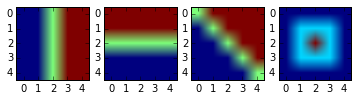
\includegraphics[width=0.5\textwidth]{./images/firstFilters.png}
	\caption{The four filters used in the first stage where the CNN was able to distinguish forest and city.}
	\label{fig:firstFilters}
\end{figure} 
\\\\
In the second phase we tried to extend our classes with the class \textit{water} or \textit{grassland}. We tried to investigate whether training only the last weights and biases were sufficient to train the network to classify three classes. During this phase we tried some adjustments to the network. We noticed that the last sub-sampling with a dimension reduction of a factor 5 could lead to problems since more information might be lost in this reduction. The underlying reasoning is that in each layer of the network more generalizations are made by the network which should represent the information of your input patch. When you downsize the feature maps at the end of the network this more contained information will be lost in this sub-sampling compared with sub-sampling earlier in the network. To test this hypothesis we trained different networks with different sub-sampling operations. Furthermore, we varied the size of the convolution kernels and the dimension of the output maps as explained in chapter \ref{chap:method}.
\\\\
From the first runs it turned out that the networks found it hard to distinguish the classes \textit{forest} and \textit{water}. By comparing some patches of both classes it became quite evident that this distinction is hard since there structure is similar (see figure \ref{fig:WaterForestPatch} ). For this reason we included the class \textit{grassland} instead of \textit{water}. From figure \ref{fig:GrassForestPatch} we can see that these patches are less similar and thus we would expect the network to perform better on these these combination of classes.


\begin{figure}[bth]
	\centering
	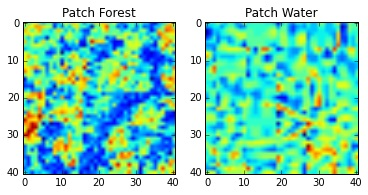
\includegraphics[width=0.5\textwidth]{./images/WaterForestPatch.jpg}
	\caption{A forest and water patch are shown. Their similarity makes it hard for the CNN to distinguish these two classes.}
	\label{fig:WaterForestPatch}
\end{figure}
\begin{figure}[bth]
	\centering
	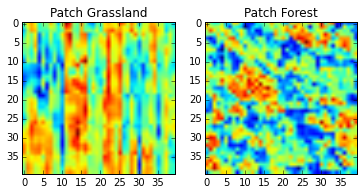
\includegraphics[width=0.5\textwidth]{./images/GrassForestPatch.jpg}
	\caption{A grassland and forest patch are shown.}
	\label{fig:GrassForestPatch}
\end{figure}

\section{Results: Cross-validation}
In this part of the research we investigated how different architectures of the network performance compared to each other. This comparison is made by using cross-validation explained in chapter \ref{chap:method}. All network had similar convolution kernels for the first layer. If we used $3$ rows or convolution kernels in the first layer we used the kernel types shown in figure \ref{fig:3filters}. For the networks with $5$ and $7$ the kernels shown in figure \ref{fig:5filters} and \ref{fig:7filters} respectively.
With equation \ref{eq:P} we calculated the performances of the networks. The classifier neuron with the highest activation value is taken to be the class of classification. If this class matches the corresponding class of the input patch the network is considered to evaluate the patch as correct else it is classified wrong. Remind, that city patches might include tree or grassland patches as well.

\begin{tiny}
\begin{center}
	\begin{tabular}{| l |p{0.75cm} |p{0.75cm} |p{0.75cm} |p{0.75cm} |p{0.75cm} |p{0.75cm} |p{0.75cm} |p{0.75cm} |p{0.75cm} |p{0.75cm} |p{0.75cm} |p{0.75cm} |p{1cm} |r | }
		\hline
		Net	& Amount of rows	& Amount of branch	& Input patch size	& First Conv. Filter size	& Pooling	& Second Conv. Filter size (random)&	Pooling	H4	&BP	&Tot. Training patches	& Crossvalidation 90\%-10\% (R/W+R)	& Forest (R/W+R)&	City (R/W+R)	& Grassland (R/W+R) \\ \hline

  \end{tabular}
\end{center}
\end{tiny}	


\begin{figure}[bth]
	\centering
	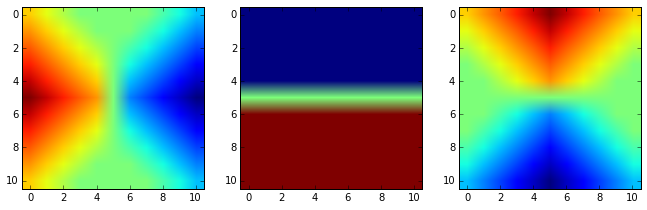
\includegraphics[width=0.3\textwidth]{./images/3filters.jpg}
	\caption{The three convolution kernels used for the architectures with three rows.}
	\label{fig:3filters}
\end{figure}

\begin{figure}[bth]
	\centering
	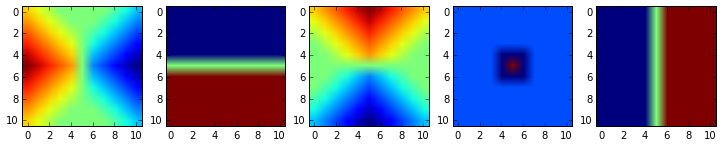
\includegraphics[width=0.5\textwidth]{./images/5filters.jpg}
	\caption{The five convolution kernels used for the architectures with five rows.}
	\label{fig:5filters}
\end{figure}

\begin{figure}[bth]
	\centering
	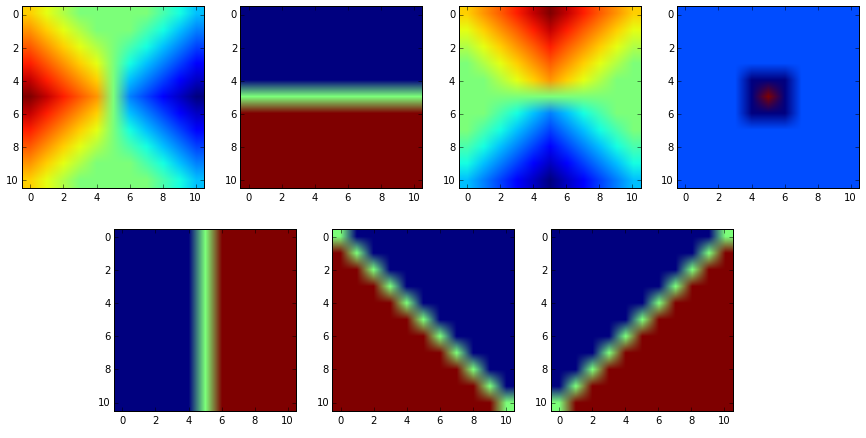
\includegraphics[width=0.4\textwidth]{./images/7filters.jpg}
	\caption{The seven convolution kernels used for the architectures with seven rows.}
	\label{fig:7filters}
\end{figure}


\chapter{Time schedule}
\begin{center}
  \begin{tabular}{| l | p{5cm}| p{5cm} | r | }
    \hline
    \textbf{Week} & \textbf{Description of work} & \textbf{Deadline} & \textbf{Labour (hours)} \\ \hline \hline
	20 & \begin{itemize} \vspace{-1.75em} \item Implement backpropagation output layer\vspace{-1em}
	\item Start examining how to take into account RGB values \vspace{-1em}
	\item Train on more pictures and examine performance on  other classes like city and water \vspace{-1em}
	\item Start developing frontend/ backend architecture
	\end{itemize}
	& Finish updated proposal & 40 					\\	\hline	
	21 &  \begin{itemize} \vspace{-1.75em} \item Work on implementing communication protocol\vspace{-1em}
	\item Experiments with connecting the nodes of the different layers of the Neural Networks \vspace{-1em}
	\end{itemize}
	& Finish backpropagation output layer, and frontend implementation of the communication protocol& 40 					\\	\hline
	22 & \begin{itemize} \vspace{-1.75em}
	\item In-between overall evaluation \vspace{-1em}
	\item Backend and frontend implementation\vspace{-1em}
	\item Experiment with preprocessed images (noise reduction) \vspace{-1em}
	\item Implement backpropagation further, until layer H3, see Figure \ref{fig:Architecture} \vspace{-1em}
	\end{itemize} & Finish model with complete RGB values and the frontend/backend architecture must be completely finished & 40 					\\  \hline
	23 & Start report writing and implement last adjustments & Finished product for demonstration & 40 	\\	\hline
	24 & Preparation for demo & Demo & 30				\\  \hline
    25 & Project finalization & - & 30 				\\ \hline
    26 & Project finalization & Project report + individual document & 40 \\ \hline
       & & & Total: 468  \\ \hline

    \hline
  \end{tabular}
\end{center}

\bibliography{Report.bib}
\bibliographystyle{apacite}

\end{document}



